\chapter{Introduction}
%\pagestyle{fancy}
%\fancyhf{}
%\rhead{
\includegraphics[width=1cm]{319th.png}}
%\lhead{\leftmark}
%\rfoot{\thepage}
%\lfoot{\footnotesize \footer{}}

\begin{center}
    \makebox[\textwidth]{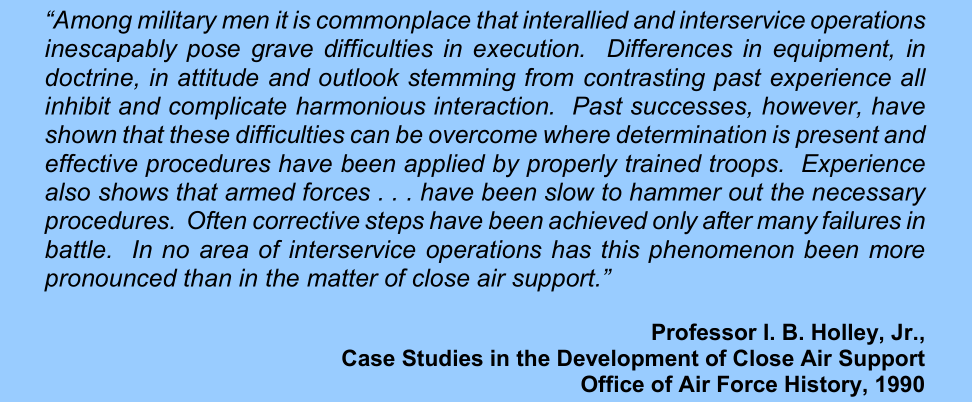
\includegraphics[width=\paperwidth]{quote1.png}}
\end{center}

\e
	
    \item 
	Bien que l'objectif principal du \acrshort{cas} soit de fournir un cadre de travail dans des conditions bien spécifiques, les techniques décrites dans ce manuel peuvent être appliquées à toute situation nécessitant un \gls{tac}.%
\ed

\section{Aperçu}

\e
    \item
    Le \acrfull{cas} est une action effectuée par des appareils à voilure fixe ou à voilure tournante contre des cibles ennemies \textbf{proches des forces amies} et nécessite une \textbf{coordination étroite} entre les missions de support aérien et le mouvement des troupes amies.
    \item
    Le \acrshort{cas} est planifié et exécuté pour appuyer les unités amies au sol. Le \acrshort{cas} est étroitement intégré au niveau du contrôle tactique des forces amies supportées. Alors que l'affectation des ressources aériennes disponibles se fait au niveau stratégique opérationnel, le processus de planification du \acrshort{cas} se fait au niveau stratégique local, pour fournir aux unités amies au contact de l'ennemi un appui-feu précis et rapide.
    \item
    Le \acrshort{cas} peut être effectué partout ou les forces amies se trouvent au contact de l'ennemi. Le mot ``rapproché'' (``Close'') n'implique pas une distance spécifique, mais plutôt un contexte. Parfois, le \acrshort{cas} peut être le meilleur moyen d'exploiter une opportunité tactique en défense ou en attaque. Le \acrshort{cas} fournit un appui-feu capable de détruire, perturber, interdire, empêcher, harceler, neutraliser ou retarder l'ennemi.
    \item
    Chaque organisation s'entraîne et emploie le \gls{cas} en tant que partie d'une coalition. Le \gls{jfc} est responsable d'intégrer ces organisations au \gls{conops} en fonctions de leurs capacités.
    \item
    Le \gls{tac} est l'autorité responsable de manœuvrer les appareils de soutien aérien et d'autoriser l'attaque finale. Un \gls{jtac} ou un \gls{faca} certifié sera reconnu comme capable et autorisé à effectuer le \gls{tac}.
    \item
    Il y a trois types de contrôle (type 1, 2 et 3):
    \ee
        \item
        Contrôle de type 1

        Le contrôle de type 1 est utilisé lorsque le \gls{jtac}/\gls{faca} a besoin de contrôler de chaque attaque individuellement ainsi que d'avoir en permanence en visuel l'appareil qui attaque ainsi que sa cible.
        \item
        Contrôle de type 2

        Le contrôle de type 2 est utilisé lorsque le \gls{jtac}/\gls{faca} a besoin de contrôler chaque attaque mais qu'il ne peut pas voir l'appareil au moment du largage ou qu'il ne peut pas voir la cible.
        \item
        Contrôle de type 3

        Le contrôle de type 3 est utilisé lorsque le \gls{jtac}/\gls{faca} a besoin de contrôler chaque engagement, avec ses restrictions, mais qu'on engagement peut être composé de plusieurs attaques.
    \end{enumerate}
    Pour plus d'informations, voyez le chapitre: \nameref{controltypes}.
    \item \gls{tgo}: le personnel effectuant les \glspl{tgo} n'ont pas l'autorité pour contrôler les appareils engagés en opération \gls{cas} ou pour autoriser le tir.
\ed
    
\section{Usage du CAS}

\e
	\item
	L'usage du \gls{cas} s'inscrit dans le \gls{conops} de par sa spécificité à pouvoir frapper des cibles inaccessibles aux troupes au sol.
	
	\item
	Le \gls{gc} garde l'autorité suprême quant à l'usage d'armement dans leur zone de contrôle.
	
	\item
	Utilité sur le champ de bataille: le \gls{cas} permet au \gls{gc} de frapper l'ennemi rapidement et de manière inattendue.
	
	\item Critères pour l'usage du \gls{cas}
	
	\ee
		\item Mission et \gls{conops}.
		\item Disposition, force et composition de l'ennemi.
		\item Capacités et limitations des appareils engagés dans le \gls{cas}.
		\item Emplacement et équipement des \gls{jtac}.
		\item \glspl{roe}.
		\item \gls{spins}.
		\item Défenses anti-aériennes ennemies et capacités alliées à les contrer.
		\item Disposition des forces amies
		\item Allocation des sorties \gls{cas}.
		\item Emplacement des civils et estimation des dommages collatéraux potentiels.	
	\ed
	
	\item Les cibles du \gls{cas} sont sélectionnées par le \gls{jtac}, en fonction des intentions du \gls{gc}, du terrain, de la météo, de la mission, des défenses ennemies, de l'armement disponible, du temps de réponse, etc. D'autres considérations peuvent entrer en ligne de compte.
\ed
	
\section{Intégration du CAS}
\e
	\item Lors des opération conjointes, l'intégration du \gls{cas} commence au niveau opérationnel. S'il est établi, le \gls{jfacc} fournit ses recommandations au \gls{jfc}. Chaque composante informe le \gls{jfc} de ses besoins et limitations. Le \gls{jfc} implémente le cadre dans lequel les opérations d'interdiction (\gls{cas}, \gls{ai}, etc.) s'intégreront dans l'\gls{opord}, l'\gls{aod}, l'\gls{ato}, l'\gls{aco} et les \gls{spins}.
\ed

\section{Emploi des voilures fixes et des voilures tournantes en opérations de CAS}

\e
	\item
	La structure organisationnelle, la mission principale et les capacités des appareils capables d'effectuer le \gls{cas} déterminent leur emploi. Bien que les \glspl{fw} et les \glspl{rw} puissent tous deux effectuer le \gls{cas}, leur emploi diffère.
	
	\item
	De par leur vitesse et leur portée opérationnelle, les \glspl{fw} offrent une grande versatilité et une grande flexibilité. De plus, ils emploient un arsenal de munitions très varié, qui peut être employé par presque toutes les conditions (météo, luminosité, ...).
	
	\item
	Les \glspl{rw} permettent de manœuvrer et de repositionner rapidement la puissance de feu en fonction de l'évolution de la situation. Ils ont un excellent temps de réponse et peuvent rester longtemps sur zone, peuvent évoluer à très faible altitude, et peuvent effectuer du \gls{cas} sur tous les types de terrain. Ils offrent également des capacités d'infiltration et d'extraction du personnel.

\ed

\section{Efficacité du CAS}

\e
	\item 
	Pour que le \gls{cas} soit efficace, il faut:
	\ee
		\item Du personnel correctement entraîné
		\item Un planning et une intégration réfléchie
		\item Un \gls{cc} efficace
		\item Une supériorité aérienne établie (tout particulièrement le \gls{sead})
		\item Une reconnaissance et une connaissance des cibles
		\item Des procédures flexibles et éprouvées
		\item De l'armement approprié
		
	\ed
\ed

\section{Définitions}

\subsection{CAS}

\e
    \item
    ``CAS'' (prononcé ``casse'') est l'abréviation de ``Close Air support'', qui signifie littéralement ``Soutien aérien rapproché''.
    \ee
        \item
        ``Soutien'', parce que l'objectif est d'augmenter la capacité d'attaque ou de défense des troupes amies au sol.
        \item
        ``Aérien'', parce que ce soutien est effectué depuis les airs, par un avion ou un hélicoptère.
        \item
        ``Rapproché'', parce que, souvent, les troupes amies sont au contact, ou sur le point de l'être, avec l'ennemi.
    \end{enumerate}
    \item
    Cette notion de ``Soutien rapproché'' est primordiale, car c'est l'essence même du CAS: la proximité des troupes amies implique une grande difficulté à classifier les cibles au sol potentielles, certainement dans un environnement en constante évolution.
    \item
    \emph{Les procédures de CAS ont été implémentées afin d'éviter, à tout prix, le tir fratricide.}
\end{enumerate}

\subsection{TAC}

\e
    \item
    ``TAC'' (prononcé ``taque'') est l'abréviation de ``Terminal Attack Control'', qui signifie littéralement ``Contrôle d'attaque terminale''. C'est l'autorité qui contrôle la manœuvre des appareils impliqués dans le CAS et qui autorise l'utilisation de l'armement.
    \item
    Dans le cadre de ce document, les deux seuls types de TAC auxquels il sera fait allusion seront le \acrshort{jtac} et le \acrshort{faca}.
\end{enumerate}

\subsection{J-TAC}
\e
    \item
    ``\acrshort{jtac}'' (prononcé ``d'jé-taque'' (EN) ou ``ji-taque'' (FR)) est l'abréviation de ``Joint Terminal Attack Controller'', qui signifie littéralement ``Contrôleur d'attaque terminale mixte/conjoint'' (le dernier mot est difficile à traduire de manière littérale).
    \ee
        \item ``Contrôleur'': lors des opérations \acrshort{cas}, c'est le \acrshort{jtac} qui est responsable de tous les aéronefs (dans sa zone).
        \item ``Attaque'': dans une zone contrôlée par un \acrshort{jtac}, aucune attaque aérienne ne peut avoir lieu sans l'autorisation de ce dernier.
        \item
        ``Terminal'': le \acrshort{jtac} se trouve toujours parmi les, ou très proche des, troupes au sol qu'il appuie. Il ne prend le contrôle du support aérien que lors de la phase d'attaque ``terminale'' du vol.
        \item
        ``Mixte/Conjoint'': le mot ``Joint'' en anglais est utilisé dans un contexte militaire lorsqu'une coalition formée de plusieurs branches armées est formée. Cela peut être, par exemple, une coalition internationale. Ce terme a toute son importance, car il est primordial que tous les \acrshort{jtac} et tous les pilotes impliqués dans le CAS parlent la même ``langue''. C'est la raison d'être du J3-09.3 et de ce document.
    \end{enumerate}
    \item Un \acrshort{jtac} sera toujours un membre du personnel formé pour occuper cette fonction.
    \item Sur le champ de bataille, en plus du contrôle des aéronefs en soutien, le \acrshort{jtac} a les responsabilités suivantes:
    \ee
        \item Connaître la situation et la position des unités amies ainsi que des composantes civiles dans la zone.
        \item Connaître les priorités du GC (``Ground commander'') qu'il soutient (-> quel est l'objectif des troupes au sol amies dans la zone ?).
        \item Approuver les cibles d'opportunités.
        \item Conseiller le GC concernant l'emploi optimal du soutien aérien.
        \item Soumettre les requêtes CAS à effet immédiat.
        \item Fournir le BDA initial
    \end{enumerate}
\end{enumerate}

\subsection{FAC(A)}

\e
    \item ``FAC(A)'' (prononcé ``faque (é)'') est l'abréviation de ``Forward Air Controller (Airborne)'', ce qui signifie littéralement ``Contrôleur aérien avancé (aéroporté)''.
    \ee
        \item ``Contrôleur'': le \acrshort{faca} est un contrôleur pour le support aérien dans une zone donnée. Son rôle précis est discuté plus en détail dans la section correspondante TODO.
        \item ``Aérien'': ce mot fait référence au fait que les unités contrôlées par le \acrshort{faca} sont des unités aériennes.
        \item ``Avancé'' : avancé signifie que le \acrshort{faca} se trouve proche des unités au sol qu'il soutient.
        \item ``Aéroporté'': contrairement au \acrshort{jtac}, le \acrshort{faca} se trouve lui même dans un aéronef.
    \end{enumerate}
\end{enumerate}

\section{Voilure fixe et voilure tournante}

\emph{(extrait traduit du JP3-09.3)}

\e
    \item
    Bien que les appareils à voilure fixe et à voilure tournante puissent tous les deux être employés pour le CAS, l'utilisation qu'il y a lieu d'en faire varie.
\end{enumerate}

\subsection{FW - Voilure fixes}

\e
    \item
    Grâce à leur vitesse et à leur rayon d'action, les appareils à voilure fixe offrent au JFC une grande versatilité et une grande flexibilité pour délivrer de l'armement où et quand c'est nécessaire.
    \item
    Les appareils à voilure fixe sont capables d'utiliser tout l'arsenal de munitions disponibles, par presque toutes les conditions météorologiques, tout particulièrement si ils sont équipés des senseurs appropriés.
\ed

\subsection{RW - Voilures tournantes}

\e
    \item Les appareils à voilure tournante offre la possibilité de manoeuvrer et repositionner la puissance de feu en réponse à une situation qui évolue en permanence.
    \item
    Les RWs disposent  d'un excellent temps de réponse et peuvent rester longtemps sur zone, peuvent naviguer et effectuer des attaques à très basse altitude, ont une capacité de CAS excellente quel que soit le terrain, et peuvent effectuer des opération de récupération et d'évacuation de personnel ou de matériel.
\ed 